\section{Analysis and Motivations}
In this section, we analyze the attention map behaviors during the generation time and illustrate how the observations motivate the adaptive attention sparse updates.

\subsection{Cross-step attention similarity}


In DLLMs, the attention compute can be formulated as:
$Out = Softmax(QK/d) V$. and the attention score can be illustrated by $Attn score = Softmax(QK/d)$. Here, $Q, K [seq,d]$, in the all steps, they are processed as the total seq = prompt+generation context. \zz{need polishing}

for different position tokens, since DLLMs will update the token by unmasking step by step, some position will generate a token and we call this step i as the "tuning point" for the position x\_i. Before this step, this position behaves as decoding, trying to denoising and find the maximal logits and after this step, this position changes to prefilling, which can provide the information for the next step token generation.

For example, referring to Figure 2, during the first two steps, the word tokens are denoised, and then performanced as the prefilling tokens in following steps.
\xz{1. figure: cross-step similarity and non-similarity case - two figures? one figure?}


To understand the attention behaviors cross steps, we first measure the attention score cosine similarity across steps. The measurement on the cosine similarity is presented in Figure xxx. Notably, the similarity between steps is \zz{}
\red{here we need to have some data to present the across-step similarity regular pattern}



\begin{figure}[h]
    \centering
    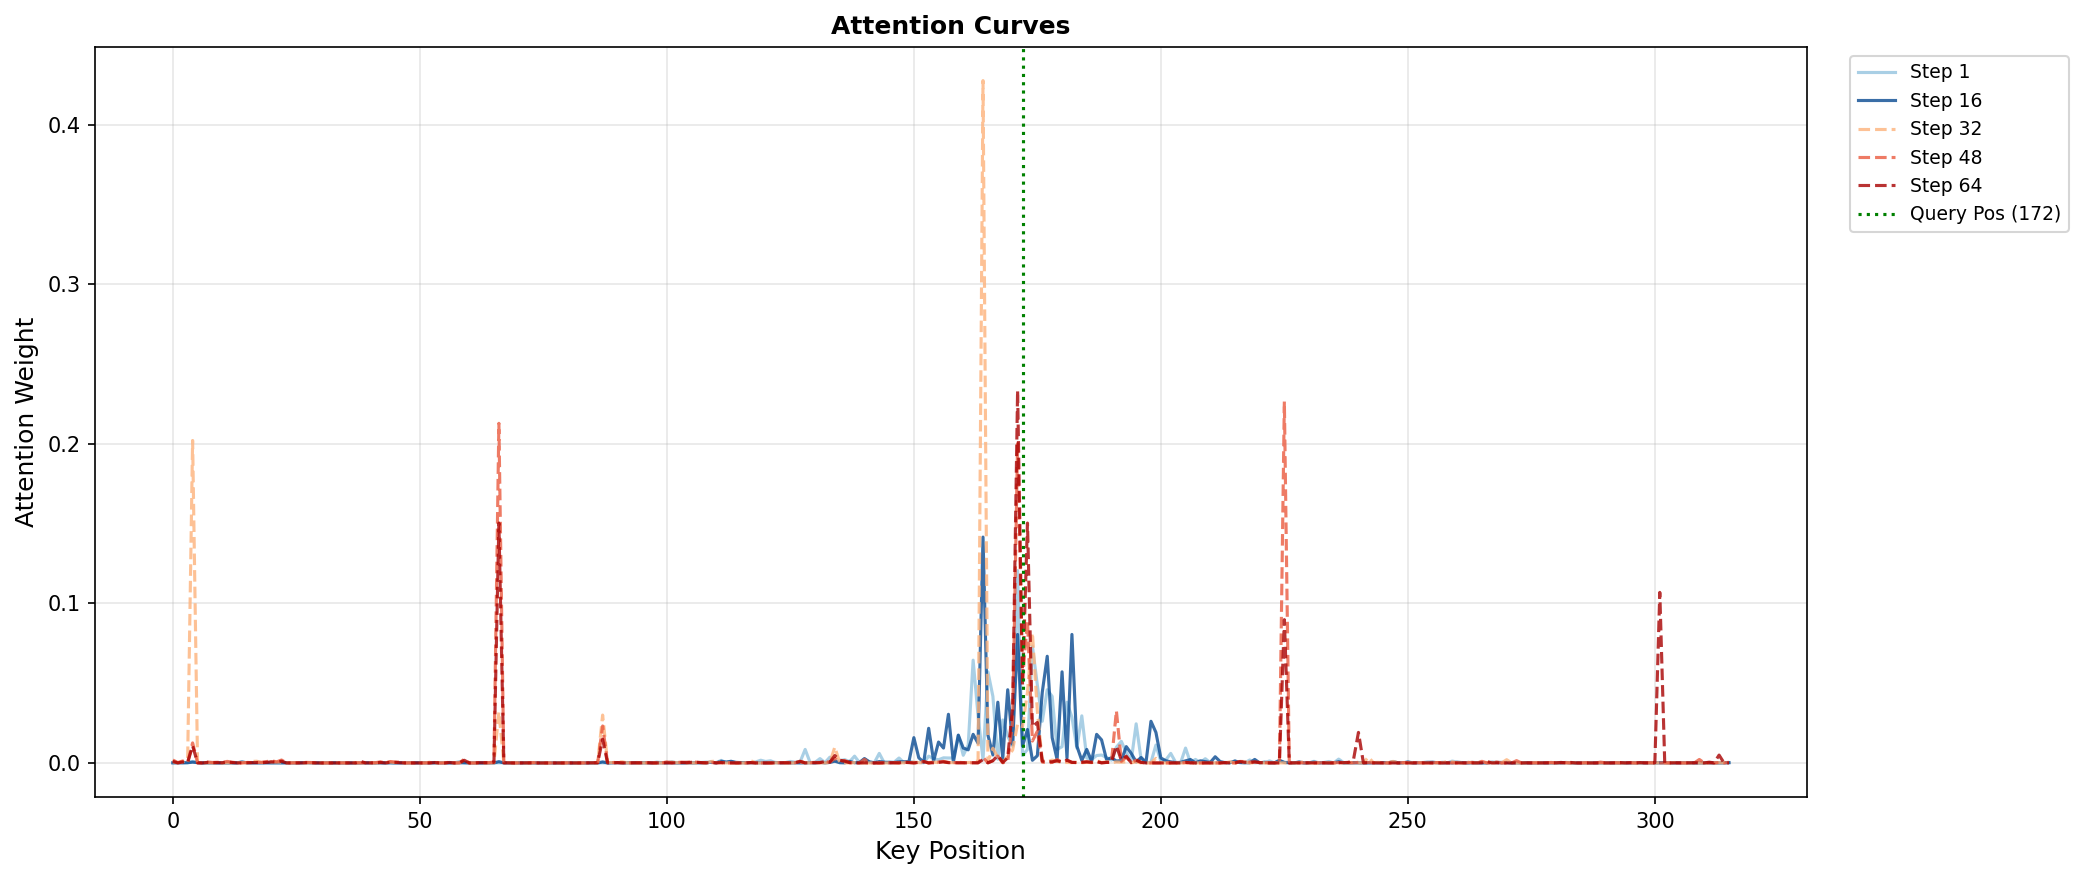
\includegraphics[width=1.0\linewidth]{figures/attn_curve_sample888_L25_H0_qpos172_steps1-16-32-48-64_combined.png}
    % \vspace{-2em} % 调整图和caption之间的距离
    \caption{cross step profiling}
    \label{fig:cross_step}
\end{figure}

\subsection{global budget sparsity}

\xz{2. figure: head-specific sparsity ratio budget}

\begin{figure}[h]
    \centering
    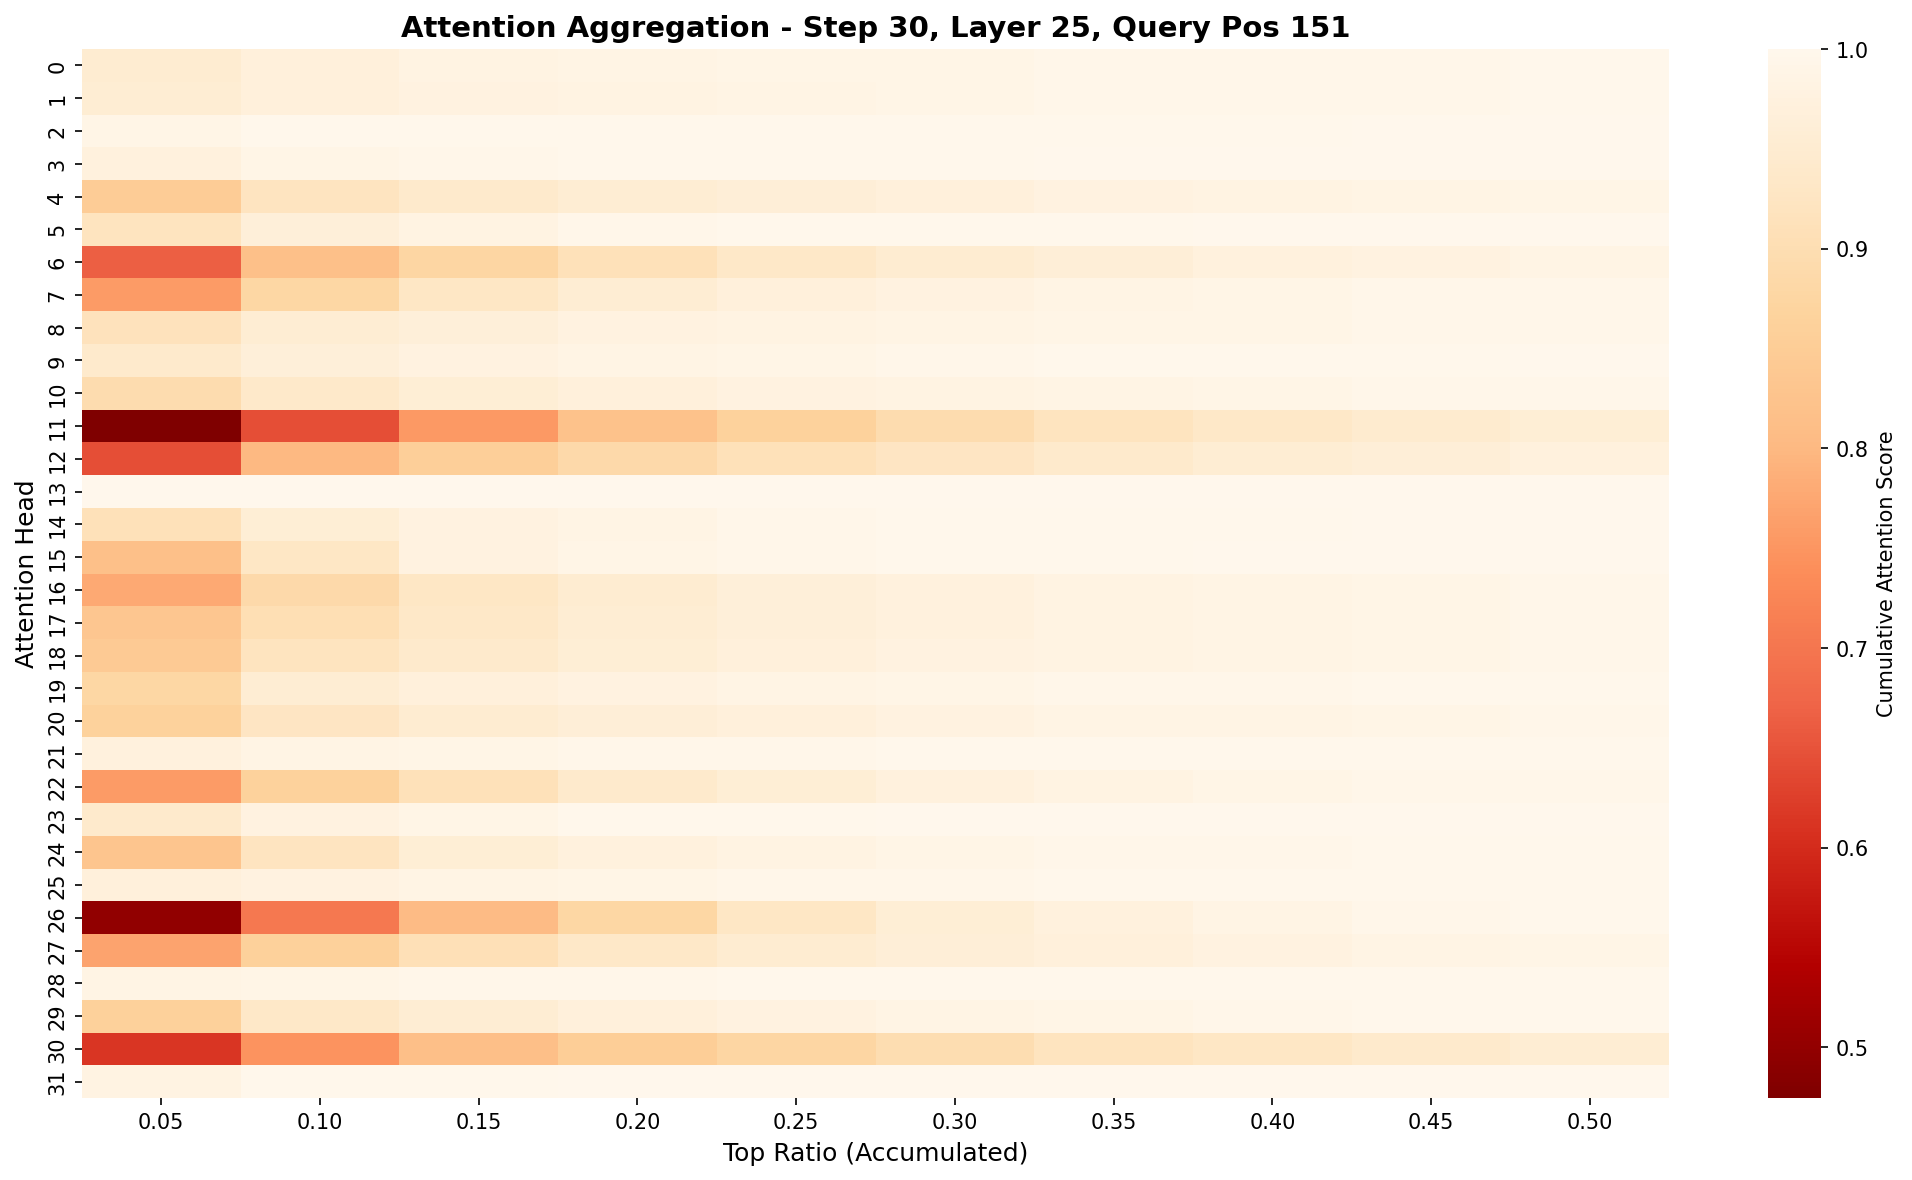
\includegraphics[width=1.0\linewidth]{figures/attention_aggregation_step30_layer25_pos151.png}
    % \vspace{-2em} % 调整图和caption之间的距离
    \caption{cross step profiling}
    \label{fig:cross_step}
\end{figure}


\section{Methodology: Step-dLLM}
In this section, we present the core methodology of Step-dLLM, which first identifies the sparse attention patterns, and then introduces step-aware adaptive sparsity mask updates last illustrate the fused kernel and implementations.

\begin{figure}[h]
    \centering
    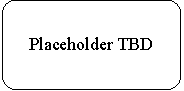
\includegraphics[width=1.0\linewidth]{figures/placeholder.pdf}
    % \vspace{-2em} % 调整图和caption之间的距离
    \caption{main figure}
    \label{fig:p}
\end{figure}

\paragraph{Step-aware sparse attention}

% Motivated by Section 3.2, we proposes a step-aware sparse mask update to reuse the similarity of sparse patterns.

% Let s be the current diffusion step and L=l+c be the total sequence length. First, we do the attention in the 
As shown in Section 3.2, the attention map between steps have some similarity. To levearage this information, we here design an algorithm to reuse the attention map cross steps. Let s be the current diffusion step and L be the total sequence length. For the attention in the selected step, we compute the flash attention and get the block wise attention map out at the fused kernel. It formulates like the fomular. Specifically, we first compute the attention output for the next ffn layer and get the mask indice by applying top-k for the block-wise 2Dmaxpool at the meanwhile

at update stage i:
\[
mask-indice, attn-output =modified-flash-attn(Q,K,V,block size,topk)
\]

then at the following steps i+1, i+2:
\[
attn out = block-sparse-attn(Q,K,V, maskindices)
\]

and then since we found that the attention score distribution is changing by the steps and the tokens will have some tuning points from denoising to steady results. To address this, we 

\paragraph{Sparsity budget across heads} DLMs exhibit head-specific attention patterns.
This makes fixed sparse patterns, e.g., the sliding-window scheme, insufficient to capture important attention scores in DLMs. To address this problem, we set the total sparsity budget for all heads, following the formulation of xxx, we 

\paragraph{Customized kernel}

To efficient cache the attention mask and do the budgeted sparse attention, we design two efficient customized kernels